\documentclass[11pt]{article}
\title{Lenses}
\author{https://github.com/heptagons/lenses}
\date{2023/12/30}

\usepackage{graphicx}

\usepackage[margin=0.75in]{geometry}
\usepackage{float} % {figure}{H}
\usepackage{amsmath} % \dfrac


%\usepackage{amssymb}
%\usepackage{subcaption}

\def\mathbi#1{\textbf{\em #1}}

\begin{document}

\maketitle
\begin{abstract}
Lenses are equilateral hexagons resembling concave and convex optical lenses. The hexagons consecutive six internal angles are $(\theta_1,\theta_2,\theta_3,\theta_1,\theta_2,\theta_3)$ where $\theta_1=X\theta_0$, $\theta_2=Y\theta_0$, and $\theta_3=Z\theta_0$ where $\theta_0 = 2\pi/S$ is the base angle of symmetry $S$.
\end{abstract}

\section{Lenses}

\section{Symmetry $5$}

Symmetry $5$ uses as base the angle $\beta = \dfrac{2\pi}5$. Includes two rhombi $\mathbi{b}$ and $\mathbi{c}$ and two lenses $\mathbi{B}$ and $\mathbi{C}$.


\subsection{Rhombi $\mathbi{b}$ and $\mathbi{c}$}

\begin{figure}[H]
\centering
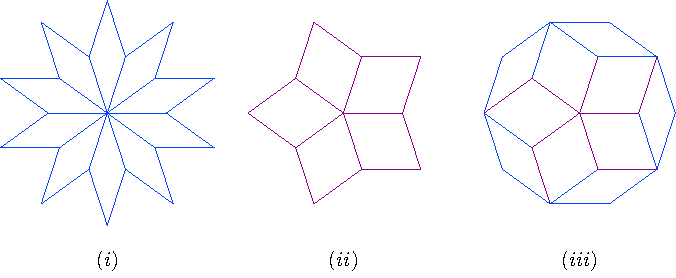
\includegraphics[scale=1.1]{bc/rhombi}
\caption{Rhombi of the types $\mathbi{b}$ and $\mathbi{c}$.}
\label{fig:bc-rhombi}
\end{figure}

Figure \ref{fig:bc-rhombi} show rhombi $\mathbi{b}$ and $\mathbi{c}$. $\mathbi{b}$ is the rhombus with smallest internal angles equal to $\dfrac{\beta}2 = \dfrac{\pi}5$. $\mathbi{c}$ is the rhombus with smallest internal angles equal to $\beta = \dfrac{2\pi}5$.
Figure $(i)$ show a dissected star whose area equals to $10\mathbi{b}$.
Figure $(ii)$ show a dissected star whose area equals to $5\mathbi{c}$.
Figure $(iii)$ show a dissected regular decagon whose area equals to $5\mathbi{b} + 5\mathbi{c}$.

\begin{figure}[H]
\centering
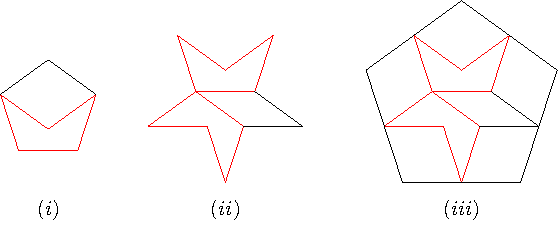
\includegraphics[scale=1.1]{bc/penta}
\caption{Regular pentagon and pentagram. Concave pentagon (in red).}
\label{fig:bc-penta}
\end{figure}

Figure \ref{fig:bc-penta} show regular pentagon and pentagram dissected with rhombi $\mathbi{b}$ and $\mathbi{c}$ and a concave pentagon (in red). We calculate the areas of the regular pentagon $P_1$ at $(i)$ and pentagram $P_G$ at $(ii)$ in function of rhombi $\mathbi{b},\mathbi{c}$. Let $x$ be the concave pentagon area. From the figures we note pentagon $P_2$ at $(iii)$ is double the side and then four times the area of pentagon $P_1$. From the figures we note the area of $P_1$ equals to $x + \mathbi{c}$ and the area of $P_2$ equals to $2x + \mathbi{b} + 5\mathbi{c}$, then we compare the pentagons and isolate $x$ to get:
\begin{align}
4P_1 &= P_2 \nonumber\\
4(x + \mathbi{c}) &= 2x + \mathbi{b} + 5\mathbi{c} \nonumber\\
x &= \frac{\mathbi{b} + \mathbi{c}}2
\end{align}
Then the areas of the pentagon and the pentagram are:
\begin{align}
P_1 &= x + \mathbi{c} 
 = \frac{\mathbi{b} + \mathbi{c}}2 + \mathbi{c}
 = \frac{\mathbi{b} + 3\mathbi{c}}2 \\
P_G &= 2x + \mathbi{b}
 = \frac{2(\mathbi{b} + \mathbi{c})}2 + \mathbi{b}
 = 2\mathbi{b} + \mathbi{c}
\end{align}

\subsection{Lenses $\mathbi{B}$ and $\mathbi{C}$}

\begin{figure}[H]
\centering
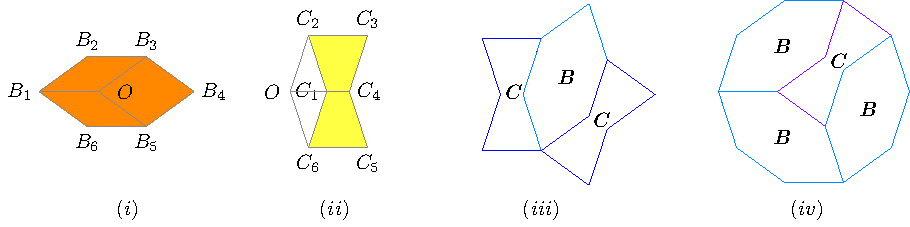
\includegraphics[scale=1.1]{bc/hexagons}
\caption{Lenses of types $\mathbi{B}$ and $\mathbi{C}$.}
\label{fig:bc-hexagons}
\end{figure}

Figure \ref{fig:bc-hexagons} show lenses $\mathbi{B}$ and $\mathbi{C}$.
Figure $(i)$ show the lense $\mathbi{B}$ with perimeter $\overline{B_1...B_6}$ which is formed adding two rhombi $\mathbi{b}$ and adding one rhombus $\mathbi{c}$ so its area equals to $2\mathbi{b} + \mathbi{c}$.
Figure $(ii)$ show the lense $\mathbi{C}$ with perimeter $\overline{C_1...C_6}$ which is formed adding two rhombi $\mathbi{c}$ and substracting one rhombus $\mathbi{b}$ so its area equals to $2\mathbi{c} - \mathbi{b}$.
Figure $(iii)$ show a dissected star whose area equals to $2\mathbi{C} + \mathbi{B} = 5\mathbi{c}$.
Figure $(iv)$ show a dissected regular decagon whose area equals to $3\mathbi{B} + \mathbi{C} = 5\mathbi{b} + 5\mathbi{c}$.



\end{document}
